%%%%%%%%%%%%%%%%%%%%%%%%%%%%%%%%%%%%%%%%%
% Beamer Presentation
% LaTeX Template
% Version 1.0 (10/11/12)
%
% This template has been downloaded from:
% http://www.LaTeXTemplates.com
%
% License:
% CC BY-NC-SA 3.0 (http://creativecommons.org/licenses/by-nc-sa/3.0/)
%
%%%%%%%%%%%%%%%%%%%%%%%%%%%%%%%%%%%%%%%%%

%----------------------------------------------------------------------------------------
%	PACKAGES AND THEMES
%----------------------------------------------------------------------------------------

\documentclass[xcolor=svgnames]{beamer}

\mode<presentation> {

% The Beamer class comes with a number of default slide themes
% which change the colors and layouts of slides. Below this is a list
% of all the themes, uncomment each in turn to see what they look like.

% \usetheme{default}
% \usetheme{AnnArbor}
% \usetheme{Antibes}
%\usetheme{Bergen}
% \usetheme{Berkeley}
% \usetheme{Berlin}
\usetheme{Boadilla}
% \usetheme{CambridgeUS}
% \usetheme{Copenhagen}
% \usetheme{Darmstadt}
% \usetheme{Dresden}
% \usetheme{Frankfurt}
% \usetheme{Goettingen}
% \usetheme{Hannover}
% \usetheme{Ilmenau}
% \usetheme{JuanLesPins}
% \usetheme{Luebeck}
% \usetheme{Madrid}
% \usetheme{Malmoe}
% \usetheme{Marburg}
% \usetheme{Montpellier}
% \usetheme{PaloAlto}
% \usetheme{Pittsburgh}
% \usetheme{Rochester}
% \usetheme{Singapore}
% \usetheme{Szeged}
% \usetheme{Warsaw}

% As well as themes, the Beamer class has a number of color themes
% for any slide theme. Uncomment each of these in turn to see how it
% changes the colors of your current slide theme.

% \usecolortheme{albatross}
% \usecolortheme{beaver}
%\usecolortheme{beetle}
% \usecolortheme{crane}
%  \usecolortheme{dolphin}
% \usecolortheme{dove}
% \usecolortheme{fly}
% \usecolortheme{lily}
% \usecolortheme{orchid}
% \usecolortheme{rose}
% \usecolortheme{seagull}
% \usecolortheme{seahorse}
% \usecolortheme{whale}
% \usecolortheme{wolverine}

% \setbeamertemplate{footline} % To remove the footer line in all slides uncomment this line
%\setbeamertemplate{footline}[page number] % To replace the footer line in all slides with a simple slide count uncomment this line

% \setbeamertemplate{navigation symbols}{} % To remove the navigation symbols from the bottom of all slides uncomment this line
}

\usepackage{graphicx} % Allows including images
\usepackage{booktabs} % Allows the use of \toprule, \midrule and \bottomrule in tables
\usepackage{tikz}
\usepackage{multicol}
\usepackage{wrapfig}
\usepackage{amsmath,amsthm,amssymb}
\usepackage{mathtools}
\usepackage{hyperref}
\DeclarePairedDelimiter\ceil{\lceil}{\rceil}
\DeclarePairedDelimiter\floor{\lfloor}{\rfloor}


\addtobeamertemplate{frametitle}{}{%
\begin{tikzpicture}[remember picture,overlay]
\node[anchor=north east,yshift=2pt] at (current page.north east) {
\includegraphics[height=0.8cm]{iiit-new.png}};
\end{tikzpicture}}

\setbeamercolor{title in head/foot}{bg=OrangeRed, fg=White}
\setbeamercolor{author in head/foot}{bg=RoyalBlue, fg=White}
\setbeamercolor{date in head/foot}{bg=SlateGray, fg=Black}

%----------------------------------------------------------------------------------------
%	TITLE PAGE
%----------------------------------------------------------------------------------------

\title[Discrete Structures]{Discrete Structures} % The short title appears at the bottom of every slide, the full title is only on the title page
\author{IIIT Hyderabad} % Your name
\institute[] % Your institution as it will appear on the bottom of every slide, may be shorthand to save space
{
Monsoon 2020 \\ % Your institution for the title page
\medskip
\textit{Tutorial 8} % Your email address
}
\date{October 14    , 2020} % Date, can be changed to a custom date
\newcommand{\comment}[1]{}
\begin{document}

\begin{frame}
\titlepage % Print the title page as the first slide
\end{frame}

\begin{frame}
\frametitle{Introduction} % Table of contents slide, comment this block out to remove it
\tableofcontents % Throughout your presentation, if you choose to use \section{} and \subsection{} commands, these will automatically be printed on this slide as an overview of your presentation
\end{frame}

%----------------------------------------------------------------------------------------
%	PRESENTATION SLIDES
%----------------------------------------------------------------------------------------

%------------------------------------------------
\section{Questions}
%------------------------------------------------

%------------------------------------------------
\subsection{Question 0}
%------------------------------------------------

\begin{frame}{Question 0}
    Each bead on a bracelet with three beads is either red, white or blue:
    \begin{figure}
        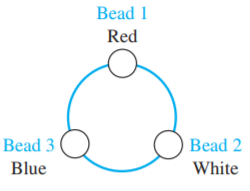
\includegraphics[width=3cm]{dstut7q5.png}
        \label{fig:my_label}
    \end{figure}
    Define the relation $R$ between bracelets as: $(B_1, B_2)$ where $B_1$ and $B_2$ are bracelets, belongs to $R$ if and only if $B_2$ can be obtained from $B_1$ by rotating it or rotating it and then reflecting it. 
    \begin{itemize}
        \item Show that $R$ is an equivalence relation
        \item What are the equivalence classes for $R$
    \end{itemize}
\end{frame}

\begin{frame}{Question 0 solution}
    Given $A = $ Set of bracelets with beads being red, white or blue \\ 
    $R = \{(B_1, B_2) | B_2 \text{ is } B_1 \text{ rotated or } B_2 \text{ is } B_1 \text{ rotated plus reflected} \}$ \\
    \textbf{Reflexive} Let $B \in A$:\\
    Bracelet $B$ is obtained by rotating $B$ by $360^\circ$. Thus $(B, B) \in R$. Thus $R$ is reflexive. \\
    \textbf{Symmetric} Let $(B_1, B_2) \in R$ \\
    If we obtained $B_2$ by rotating by $x^\circ$, then we can obtain $B_1$ from $B_2$ by rotating $x^\circ$ in the opposite direction. If we have obtained $B_2$ by rotating by $x^\circ$ and then reflecting, then we can obtain $B_1$ by rotating $x^\circ$ in the opposite direction and then reflecting. Thus $(B_2, B_1) \in R$. Thus $R$ is symmetric.\\
    \textbf{Transitive} Let $(B_1, B_2), (B_2, B_3) \in R$ \\
    If $B_2$ is obtained by rotation by $x^\circ$ and $B_3$ is obtained by rotation by $y^\circ$. Then to obtain $B_3$ from $B_1$ we rotate by $(x + y)^\circ$ and then applying the respective reflections. Thus $R$ is transitive.\\
    $R$ is an equivalence relation
\end{frame}

\begin{frame}{Question 0 solution - 2}
    Each bead can take on three colors: $W$ White, $R$ Red, $B$ Blue. \\
    The equivalence classes from bracelet $B$ contain all bracelets that can be obtained by rotating/reflecting bracelet $B$, which means the bracelets contain the same colors but the ordering will be different. \\
    $[RRR]_R = \{RRR\}$ \\
    $[WWW]_R = \{WWW\}$ \\
    $[BBB]_R = \{BBB\}$ \\
    $[BBR]_R = \{BBR, BRB, RBB\}$ \\
    $[BBW]_R = \{BBW, BWB, WBB\}$ \\
    $[WWR]_R = \{WWR, WRW, RWW\}$ \\
    $[WWB]_R = \{WWB, WBW, BWW\}$ \\
    $[RRB]_R = \{RRB, RBR, BRR\}$ \\
    $[RRW]_R = \{RRW, RWR, WRR\}$ \\
    $[BRW]_R = \{BRW, BWR, RWB, RBW, WRB, WBR\}$
\end{frame}


%------------------ ------------------------------
\subsection{Question 1}
%------------------------------------------------

\begin{frame}{Question 1}
    \textbf{1.1} Let $R$ be the relation $\{(a, b) | a \text{ divides } b\}$ on the set of integers. What is the symmetric closure of $R$? \\
    \textbf{1.2} Let $R$ be the relation $\{(a, b) | a \neq b \}$ on the set of integers. What is the reflexive closure of $R$? \\
    \textbf{1.3} Let $R$ be the relation $\{(a, b) | a > b \}$ on the set of positive integers. Find the smallest relation containing $R$ that is both reflexive and symmetric? \\
\end{frame}

\begin{frame}{Question 1 Solutions}
    \textbf{1.1} To form the symmetric closure of $R$ we need to add all pairs $(b, a)$ such that $(a, b)$ is in $R$. In this case, that means that we need to include pairs $(b, a)$ such that $a$ divides $b$, which is equivalent to saying that we need to include all the pairs $(a, b)$ such that $b$ divides $a$. Thus the closure is $\{ (a, b) | a \text{ divides } b \text{ or } b \text{ divides } a \}$ \\
    \textbf{1.2} To form the reflexive closure we have to get $R \cup \bigtriangleup$ i.e. $R \cup \{(a, b) | a = b\}$. Thus we will get $R = \{(a, b) | a \neq b \vee a = b\}$ \\
    \textbf{1.3} The reflexive closure is $R = \{(a, b) | a \geq b\}$. The symmetric closure is $R = \{(a, b) | a \neq b\}$. The smallest possible is when $a, b \in \mathbb{Z}^+$. Thus the answer is $\mathbb{Z}^+ \times \mathbb{Z}^+$
\end{frame}


%------------------------------------------------
\subsection{Question 2}
%------------------------------------------------

\begin{frame}{Question 2}
    \small{
        \textbf{2.1} Determine which of the following relations $f$ are functions from set $X$ to set $Y$:
        \begin{enumerate}
            \item $X = \{[-2, 1, 0, 1, 2\}$, $Y=\{-3, 4, 5\}$ and $f =\{(-2, -3), (1, 4), (2, 5)\}$
            \item $X = Y = \{-3, 1, 0, 2 \}$ and $f = \{(-3, -1), (0, 2), (2, -1), (-3, 0), (-1, 2)\}$
            \item $X = Y = \text{ the set of all integers}$, and $f = \{(a, b) \in \mathbb{Z} \times \mathbb{Z} | b = \sqrt{a}\}$
            \item $X = Y = \text{ the set of all integers}$, and $f = \{(a, b) \in \mathbb{Z} \times \mathbb{Z} | b = a + 1\}$
        \end{enumerate}
        \textbf{2.2} Determine which of the following functions are one-one, onto or both? 
        \begin{enumerate}
            \item $f: \mathbb{N} \rightarrow \mathbb{Z} - \{0\}$ defined by $f(n) = -n$ for all  $n \in N$
            \item $f: \mathbb{R} \rightarrow \mathbb{R}$ defined by $f(x) = |x| + x$ for all $x \in \mathbb{R}$
            \item $f: \mathbb{C} \rightarrow \mathbb{R}$ defined by $f(z) = |z|$ for all $z \in \mathbb{C}$
            \item $f: \mathbb{R} \rightarrow \mathbb{R}$ defined by $f(x) = x^2$ for all $x \in \mathbb{R}$
        \end{enumerate}
    }
\end{frame}

\begin{frame}{Question 2 solutions}
    \textbf{2.1}
    \begin{itemize}
        \item The domain of $f$, $D(f) = \{-2, 1, 2\} \neq X$. Hence $f$ is not a function $X$. 
        \item We have $(-3, 1)$ and $(-3, 0)$, so $f$ is not a function
        \item We have $\sqrt{2} \neq \in \mathbb{Z}$. Thus $f$ is not a function.
        \item It is a function
    \end{itemize}
    \textbf{2.2}
    \begin{itemize}
        \item $f$ is one-one, but not onto.
        \item $f$ is not one-one, because for negative numbers this is $0$. $f$ is not onto because no negative. 
        \item $f$ is not onto because it gives only $R^+ \cup \{0\}$. $f$ is not one-one.
        \item $f$ is not one-one. $f$ is not onto.
    \end{itemize}
\end{frame}


%------------------------------------------------
\subsection{Question 3}
%------------------------------------------------

\begin{frame}{Question 3}
    \textbf{3.1} Let $f$ be a function from the set $\mathbb{N}$ into the set $X = \{0, 1, 2, 3, 4, 5, 6, 7, 8\}$ defined by $f(x) = x \text{(mod 7)}$ for $x \in \mathbb{N}$. Find $Im(f)$. Is $f$ onto $X$? Is $f$ one-one? \\
    \textbf{3.2} For what domain and co-domain will the function $f(x) = \floor{\sqrt{n}}$ be one-one and onto? \\
\end{frame}

\begin{frame}{Question 3 solutions}
    \textbf{3.1} We get $n = 7t + r$, $0 \leq r \leq 7$. Thus the image of $f$ is $\{0, 1, 2, 3, 4, 5, 6\}$. Also $f$ is not one-one because many numbers give the same remainder.\\ 
    \textbf{3.2} If we have domain as $S = \{x | x \text{ is a perfect square}\}$. If we have codomain as $\mathbb{Z}$ then we will have co-domain = range.
\end{frame}

%------------------------------------------------
\section{BONUS}
%------------------------------------------------

\begin{frame}{BONUS}
    \begin{alertblock}{NOTE:}
        \textit{The following content is additional, and present to round out the discussion on closures. No need to invest time to this as you will learn this properly in Graph Theory. This was not taught in the lectures.}
    \end{alertblock}
\end{frame}

\begin{frame}{Relations as Matrices}
    \begin{definition}
        Suppose $R$ is a relation from $A = \{a_1, a_2, \ldots, a_m\}$ to $B=\{b_1, b_2, \ldots, b_n\}$, then the relation $R$ can be represented by a matrix $\boldsymbol{M}_R = [m_{ij}]$, where
        \[
            m_{ij} = 
            \begin{cases}
                1 & \text{ if } (a_i, b_j) \in R \\
                0 & \textbf{ if } (a_i, b_j) \notin R \\
            \end{cases}
        \]
        \textbf{Such representation depends upon the ordering of $A$ and $B$} \\
        \textbf{Such representations make sense when both $A$ and $B$ are finite.}
    \end{definition}
\end{frame}

\begin{frame}{Relations as Matrices - 2}
    The matrix of a relation on a set, which is a \underline{square matrix} is very useful to determine certain properties of the relation.
    \begin{itemize}
        \item If $R$ is reflexive, then $\boldsymbol{M_{ii}} = 1$ for all $i = 1, 2, 3, \ldots, n$
        \item if $R$ is symmetric, then $\boldsymbol{M_R} = \boldsymbol{(M_R)^t}$
        \item $\boldsymbol{M_{R_1 \cup R_2}}  = \boldsymbol{M_{R_1}} \vee \boldsymbol{M_{R_2}}$
        \item $\boldsymbol{M_{R_1 \cap R_2}}  = \boldsymbol{M_{R_1}} \wedge \boldsymbol{M_{R_2}}$
        \item $\boldsymbol{M_{S \circ R}} = \boldsymbol{M_R} \odot \boldsymbol{M_S}$
        \item $\boldsymbol{M_{R^n}} = \boldsymbol{(M_R)^n}$
    \end{itemize}
\end{frame}

\comment{\begin{frame}{Relations as Directed Graphs}
    \begin{definition}
        A directed graph $G = (V, E)$ is defined as such with $V$ nodes and $E$ edges between the nodes. Directed graph implies that the edges are directional and have a starting node and terminating node. \\
        We may also represent a relation using directed graph. If there exists a relation $R$ between $A$ and $B$, all the nodes of the graph would be the elements from the set $A \cup B$. If $(a, b) \in R$, then there would be an edge from the node $a$ to node $b$ in the directed graph.
    \end{definition}
\end{frame}
}
\begin{frame}{Relationship between matrix and DGs}
    \centering
    The matrix representation and the graph representation are interchangeable, and the matrix representation is called the \textbf{\underline{Adjacency Matrix}} of the directed graph.
    \begin{figure}
        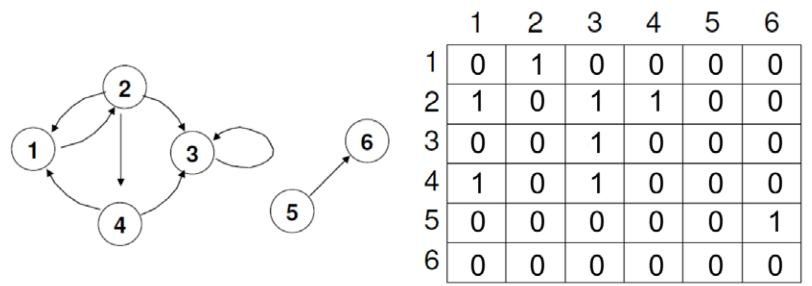
\includegraphics[width=0.95\linewidth]{A-directed-graph-represented-by-an-adjacency-matrix.png}
        \caption{An example of matrix and graph relation}
        \label{fig:my_label}
    \end{figure}
\end{frame}

\begin{frame}{Paths in a directed graph}
    A path between $a$ and $b$ is a sequence of edges that are followed starting from $a$ to finally reach $b$. The path length is given by the number of edges traversed to reach $b$. We are generally interested in minimum path lengths. It is possible that no path may exist between $a$ and $b$. 
    \begin{block}{Theorem}
        Let $R$ be a relation on a set $A$. There is a path of length $n$, where $n$ is a positive integer, from $a$ to $b$ iff $(a, b) \in R^n$.
    \end{block}
\end{frame}

\begin{frame}{Connectivity Relation and Transitive Closure}
    \begin{definition}
        Let $R$ be a relation on a set $A$. The connectivity relation $R^*$ consists of the pairs $(a, b)$ such that there is a path of length at least one from $a$ to $b$ in $R$
        \[
            R^* = \bigcup_{n=1}^\infty R^n
        \]
    \end{definition}
    \begin{block}{Theorem}
        The transitive closure of a relation $R$ equals the connectivity relation $R^*$
    \end{block}
\end{frame}

\begin{frame}{How to find closures for relations on finite set}
    If we have a relation $R$ such that \textbf{we can construct a square matrix} $\boldsymbol{M_R}$ for the relation, then: 
    \begin{itemize}
        \item Reflexive Closure: 
        \[
            \boldsymbol{M_{R \cup \bigtriangleup}} = \boldsymbol{M_R} \vee \boldsymbol{I_n}
        \]
        \item Symmetric Closure:
        \[
            \boldsymbol{M_{R \cup R^{-1}}} = \boldsymbol{M_R} \vee \boldsymbol{(M_R)^t}
        \]
        \item Transitive Closure:
        \[
            \boldsymbol{M_{R^*}} = \boldsymbol{M_R} \vee \boldsymbol{M_R^{[2]}} \vee \boldsymbol{M_R^{[3]}} \vee \ldots \vee \boldsymbol{M_R^{[n]}} 
        \]
    \end{itemize}
\end{frame}

\begin{frame}{Bonus Question}
    Using the method shown above, find the reflexive, symmetric and transitive closures for the relations on $\{1, 2, 3, 4\}$
    \begin{enumerate}
        \item $\{(1, 2), (2,1), (2,3), (3,4), (4,1)\}$
        \item $\{(1, 2), (1,3), (1,4), (2,3), (2,4), (3, 4)\}$
    \end{enumerate}
\end{frame}

\end{document} 